\section{Approach Upgrade}

	\begin{frame}
		\frametitle{NMPC with Switching Objective}
		\onslide<1->
		{
			\begin{block}{Optimization Problem}
				\parbox[c][3\baselineskip][t]{\textwidth}{
					\begin{align*}
					\underset{\vartheta^*,\mathbf{U}^*}{\text{min    }}
					J_{N_p}(\vartheta_k) = (1 - \tikzmark{a16}\beta_2 - \tikzmark{a17}\beta_3) \times J_1 + 
					\tikzmark{a18}\beta_2 \times J_2 - \tikzmark{a19}\beta_3 \times J_3
					\end{align*}
				}
			\end{block}
		}
		\onslide<3->
		{Objectives:}
		\begin{itemize}
			\onslide<4->
			{\item $J_1 = w_1 \times \tikzmark{a20}\ell_{p,1}(\cdot,\cdot)\tikzmark{a21}$}
			\onslide<5->
			{\item $J_2 = w_2 \times J_1 + \tikzmark{a22}J_4$}
			\onslide<7->
			{\item $J_3 = w_3 \times J_1 + \tikzmark{a23}J_5$ \\ [0.7cm]}
		\end{itemize}
		\onslide<9->
		{
			\[
			J_{N_p}(\vartheta_k) = 
			\begin{cases}
			\beta_2 = 0, \enspace \beta_3 = 1, 				& \text{if a dynaminc obstacle is detected} \\
			\beta_2 = 1, \enspace \beta_3 = 0, 				& \text{else, if the robot is near the goal} \\
			\beta_2 = 0, \enspace \beta_3 = 0, 				& \text{otherwise} 
			\end{cases}
			\]
		}
		\begin{tikzpicture}[overlay, remember picture]
		\coordinate (A16) at ($({pic cs:a16})+(1ex, 0.5ex)$);
		\coordinate (A17) at ($({pic cs:a17})+(1ex, 0.5ex)$);
		\coordinate (A18) at ($({pic cs:a18})+(1ex, 0.5ex)$);
		\coordinate (A19) at ($({pic cs:a19})+(1ex, 0.5ex)$);
		\coordinate (A20) at ($({pic cs:a20})+(0ex, 1.8ex)$);
		\coordinate (A21) at ($({pic cs:a21})+(-0.1ex, -0.6ex)$);
		\coordinate (A22) at ($({pic cs:a22})+(1ex, 0.5ex)$);
		\coordinate (A23) at ($({pic cs:a23})+(1ex, 0.5ex)$);
		\onslide<2->{
			\node [fit=(A16), draw=tugreen, circle, thick, inner sep=4.5pt] (n16) {};
			\node [fit=(A17), draw=tugreen, circle, thick, inner sep=4.5pt] (n17) {};
			\node [fit=(A18), draw=tugreen, circle, thick, inner sep=4.5pt] (n18) {};
			\node [fit=(A19), draw=tugreen, circle, thick, inner sep=4.5pt] (n19) {};
			\node[overlay, below of= n16, node distance = 4em] at (8.5,5.2) (t16) {Binary};
			\node[overlay, below of= t16, node distance = 1em] (t16_1) {Multipliers};
			\draw [thick, -latex, tugreen] (n16.south) to [above] (t16.north);
			\draw [thick, -latex, tugreen] (n17.south) to [above] (t16.north);
			\draw [thick, -latex, tugreen] (n18.south) to [above] (t16.north);
			\draw [thick, -latex, tugreen] (n19.south) to [above] (t16.north);
		}
		\onslide<4->{
		\node [fit=(A20)(A21), draw=tugreen, rounded corners, thick, inner sep=1pt] (n20) {};
		\node[overlay, right of= n20, node distance = 7.5em] (t20) {Euclidean distance};
		\draw [thick, -latex, tugreen] (n20.east) to [left] (t20.west);
		}
		\onslide<6->{
		\node [fit=(A22), draw=tugreen, circle, thick, inner sep=4.5pt] (n22) {};
		\node[overlay, right of= n22, node distance = 9em] (t22) {Reference orientation: $\ell_{p,3}(\cdot,\cdot)$};
		\draw [thick, -latex, tugreen] (n22.east) to [left] (t22.west);
		}
		\onslide<8->{
		\node [fit=(A23), draw=tugreen, circle, thick, inner sep=4.5pt] (n23) {};
		\node[overlay, right of= n23, node distance = 7.4em] (t23) {Dyn Obstacle Objective};
		\draw [thick, -latex, tugreen] (n23.east) to [left] (t23.west);
		}
		\end{tikzpicture}
	\end{frame}
	
	\begin{frame}
		\frametitle{NMPC Control Loop with Switching Objective}
		\centering
		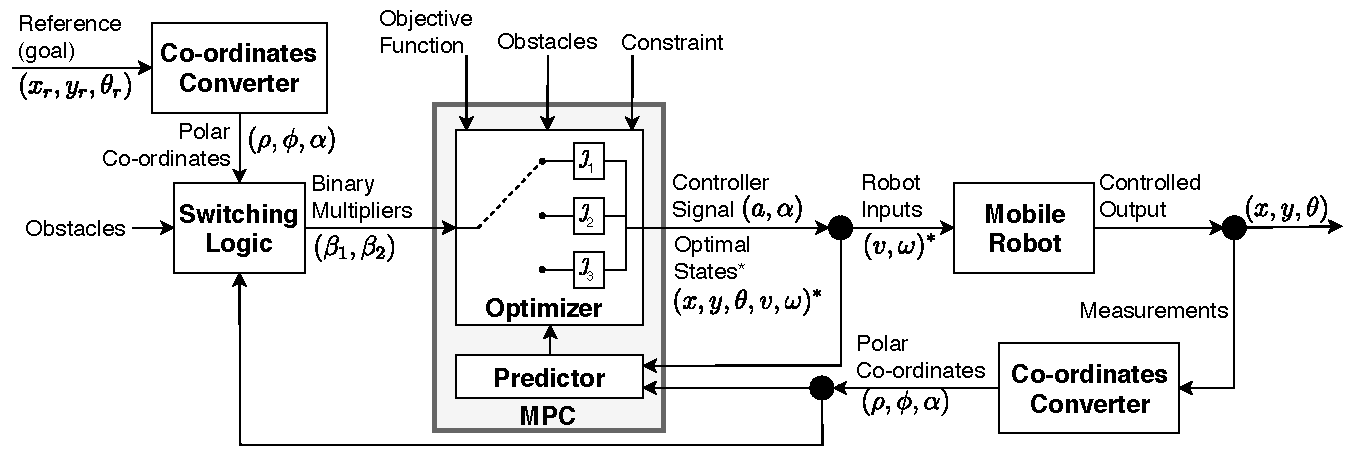
\includegraphics[scale=0.65]{pictures/block_diagram_polar_switch_1.pdf}
	\end{frame}

	\begin{frame}
		\frametitle{Scenario \textrm{IV}: State Trajectory Evolution}
		\begin{columns}[T]
			\only<1>{
				\begin{column}{0.49\textwidth}
					\centering
					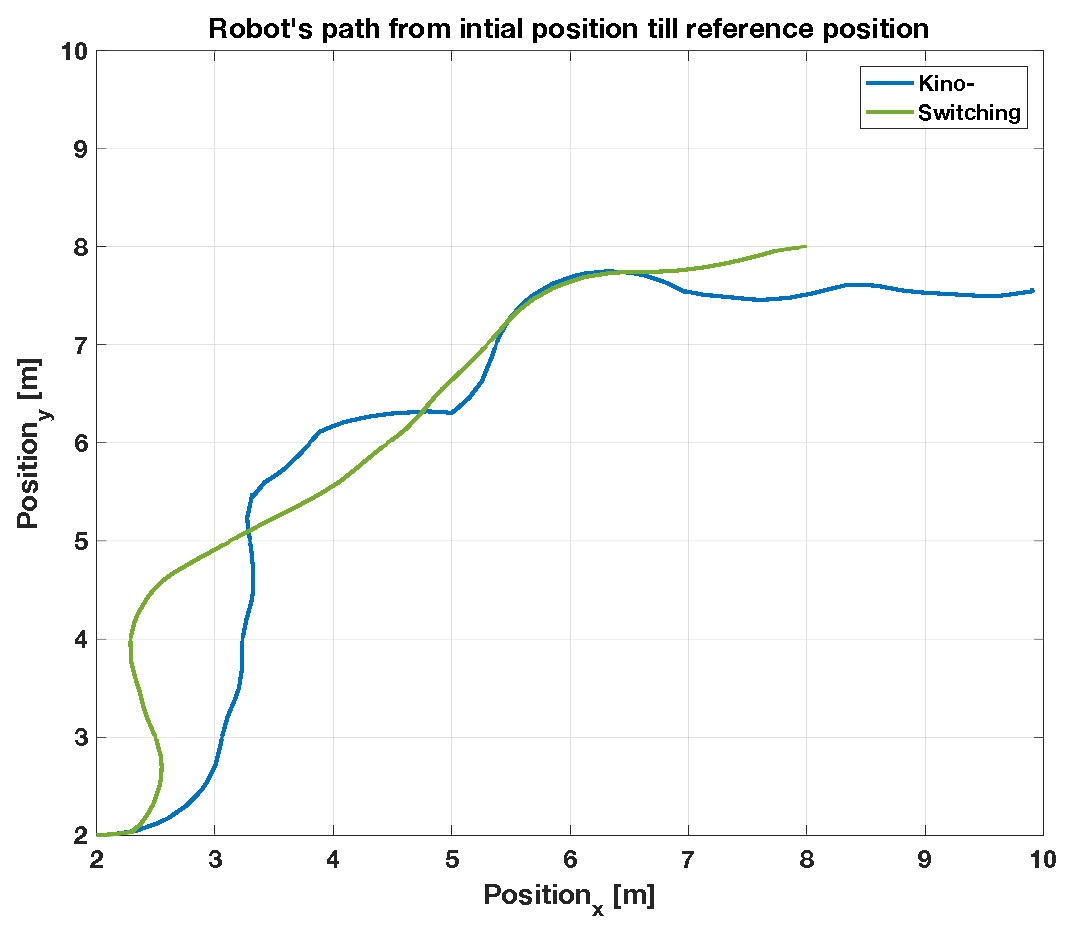
\includegraphics[scale=0.46]{pictures/graphs/sn3_group/sn3_states_p.eps}
				\end{column}
			}
			\only<2>{
				\begin{column}{0.49\textwidth}
					\centering
					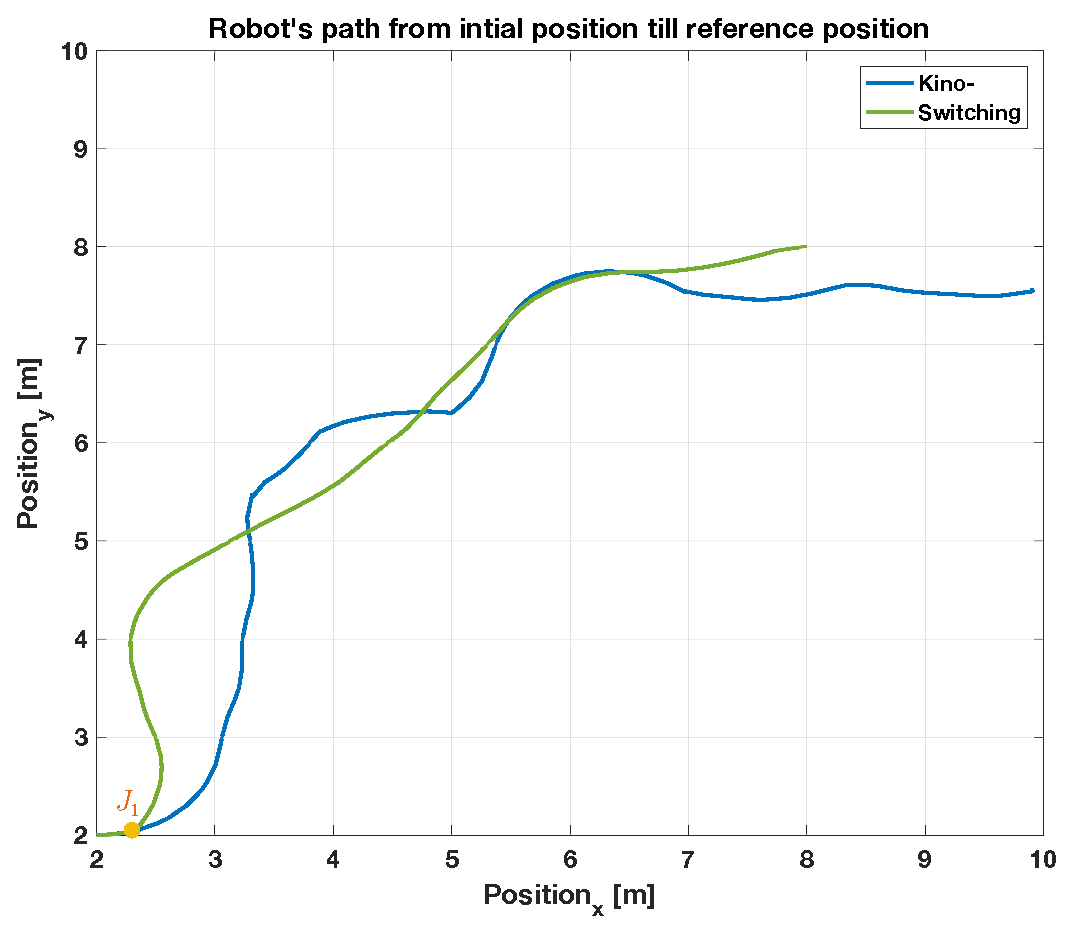
\includegraphics[scale=0.46]{pictures/graphs/sn3_group/sn3_states_p_1.eps}
				\end{column}
			}
			\only<3>{
				\begin{column}{0.48\textwidth}
					\centering
					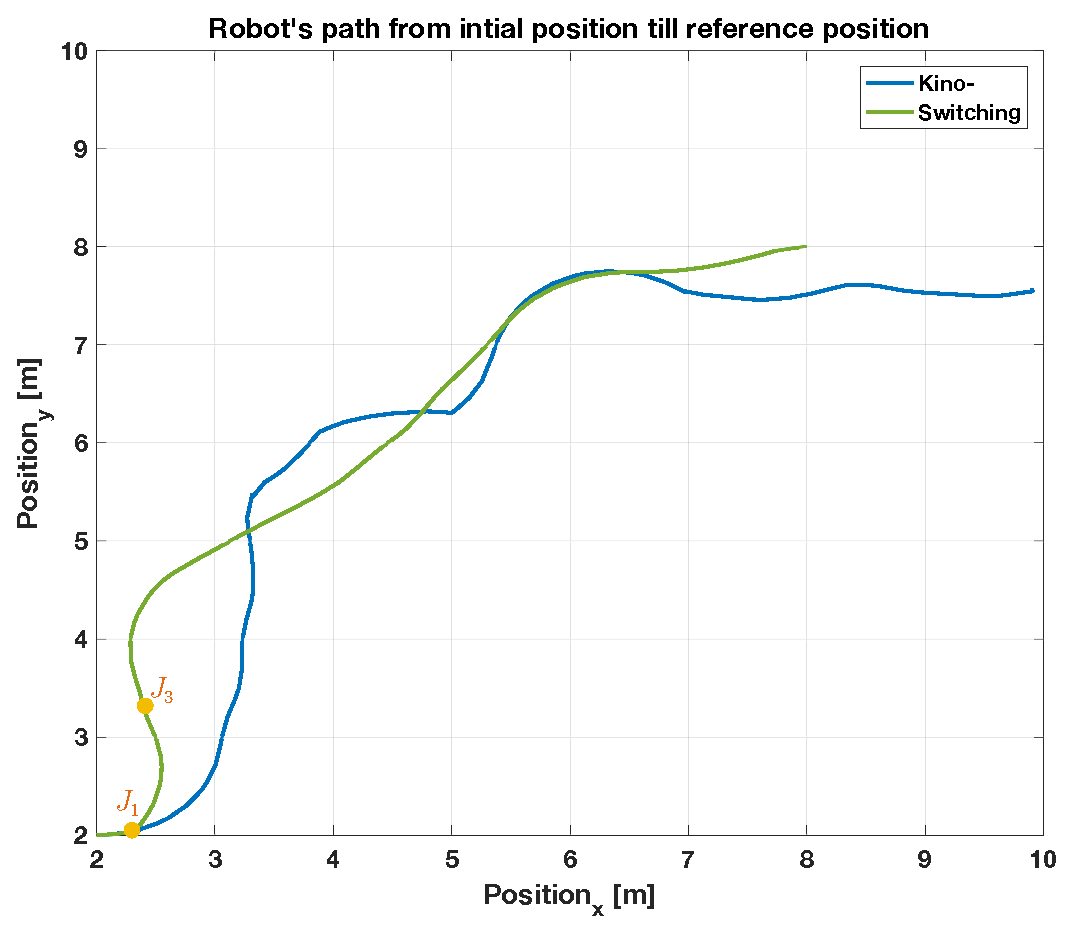
\includegraphics[scale=0.46]{pictures/graphs/sn3_group/sn3_states_p_2.eps}
				\end{column}
			}
			\only<4>{
				\begin{column}{0.49\textwidth}
					\centering
					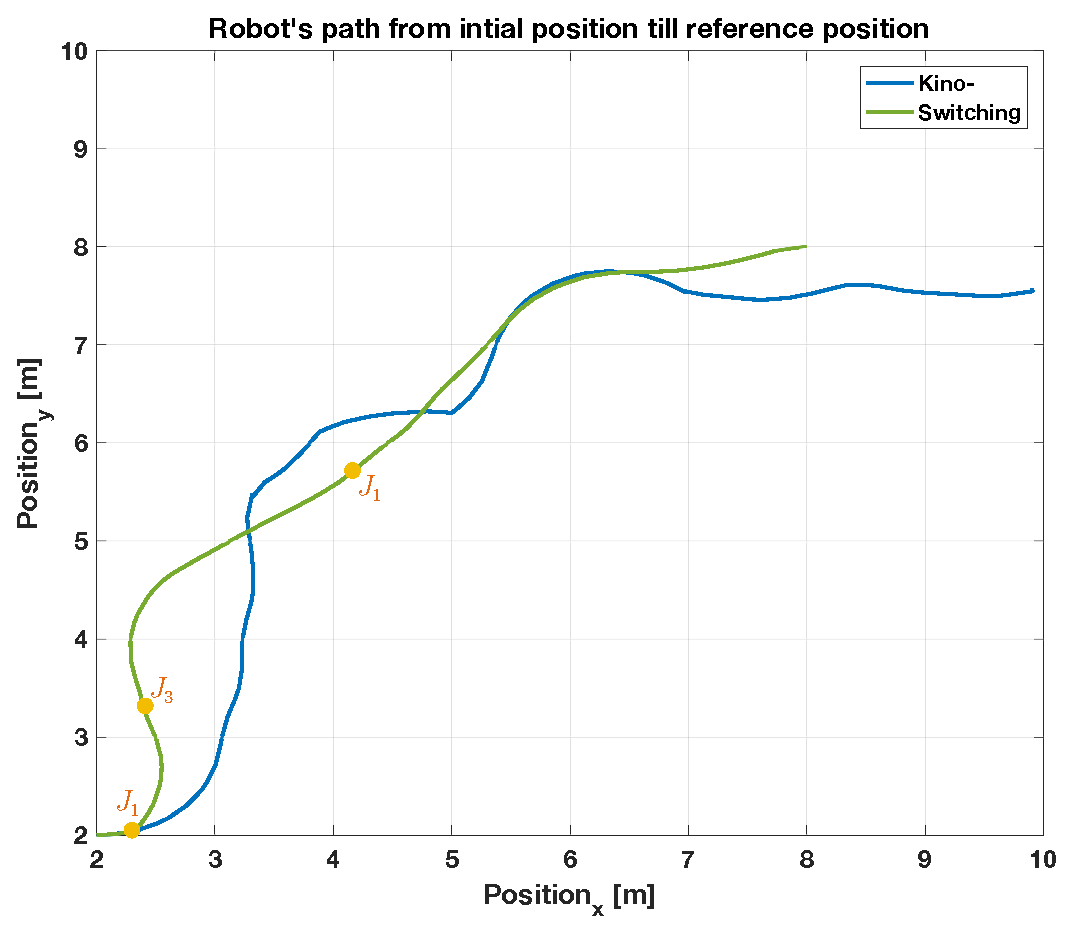
\includegraphics[scale=0.46]{pictures/graphs/sn3_group/sn3_states_p_3.eps}
				\end{column}
			}
			\only<5>{
				\begin{column}{0.49\textwidth}
					\centering
					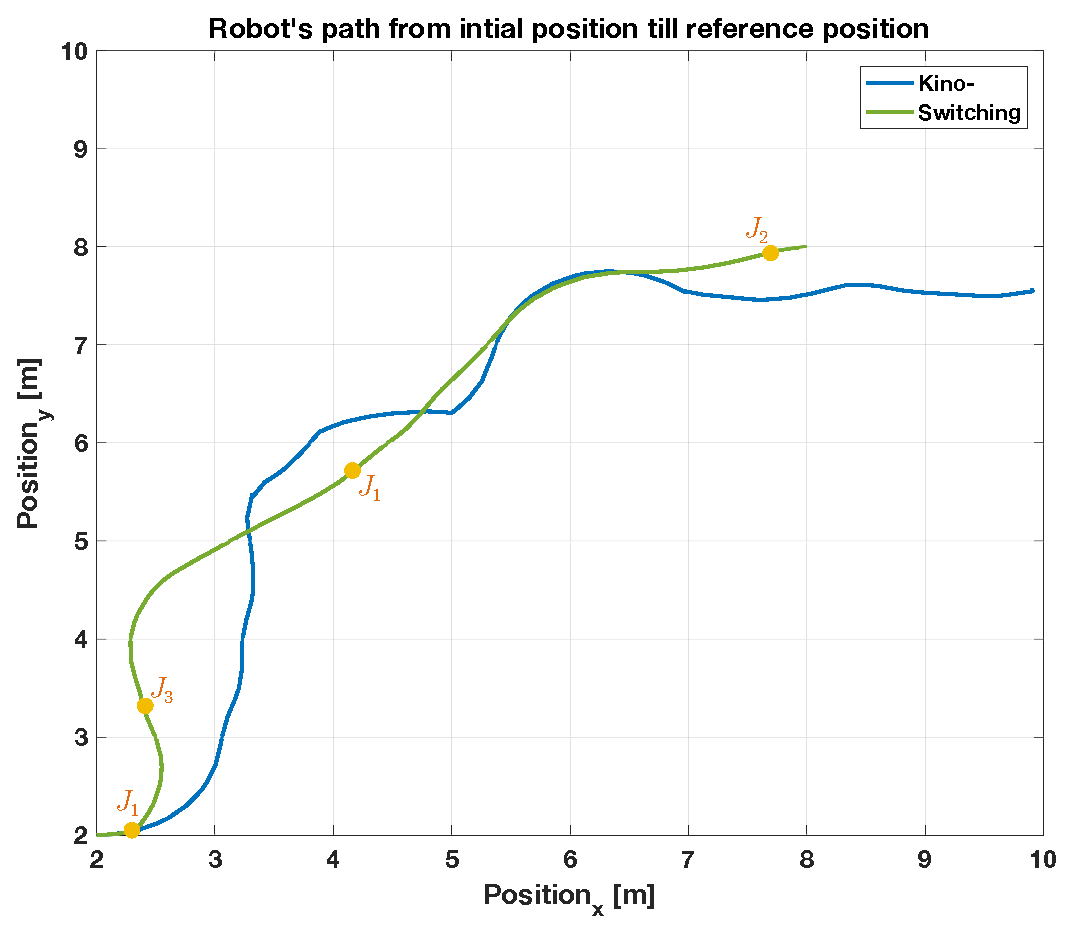
\includegraphics[scale=0.46]{pictures/graphs/sn3_group/sn3_states_p_4.eps}
				\end{column}
			}
		
			\only<1>{
				\begin{column}{0.46\textwidth}
					\centering
					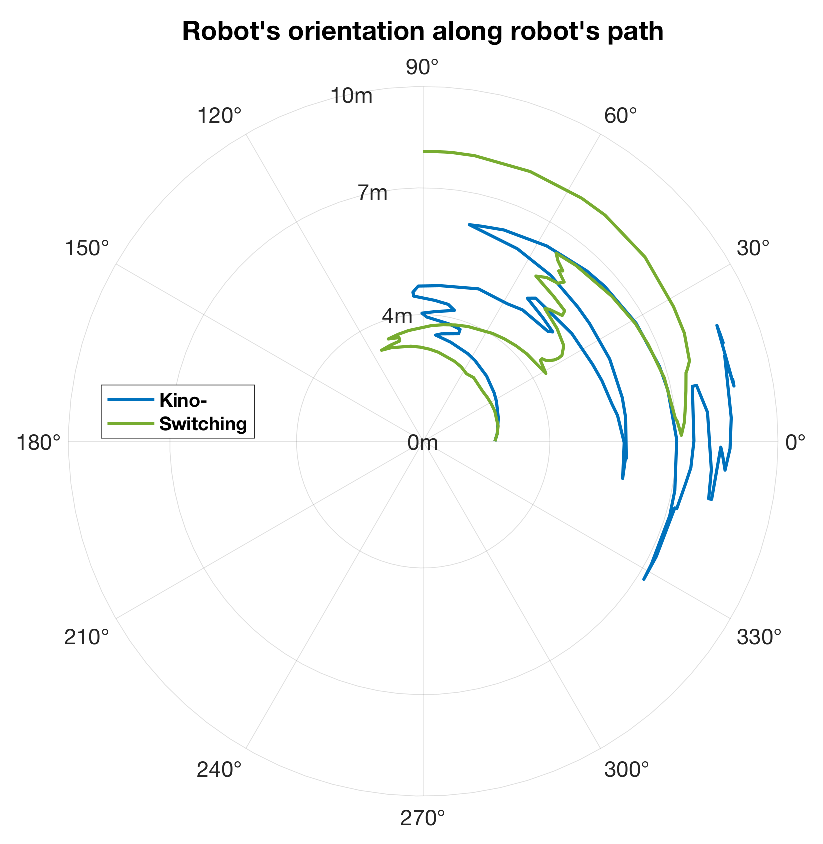
\includegraphics[scale=0.49]{pictures/graphs/sn3_group/sn3_states_pa.eps}
				\end{column}
				}
			\only<2>{
				\begin{column}{0.48\textwidth}
					\centering
					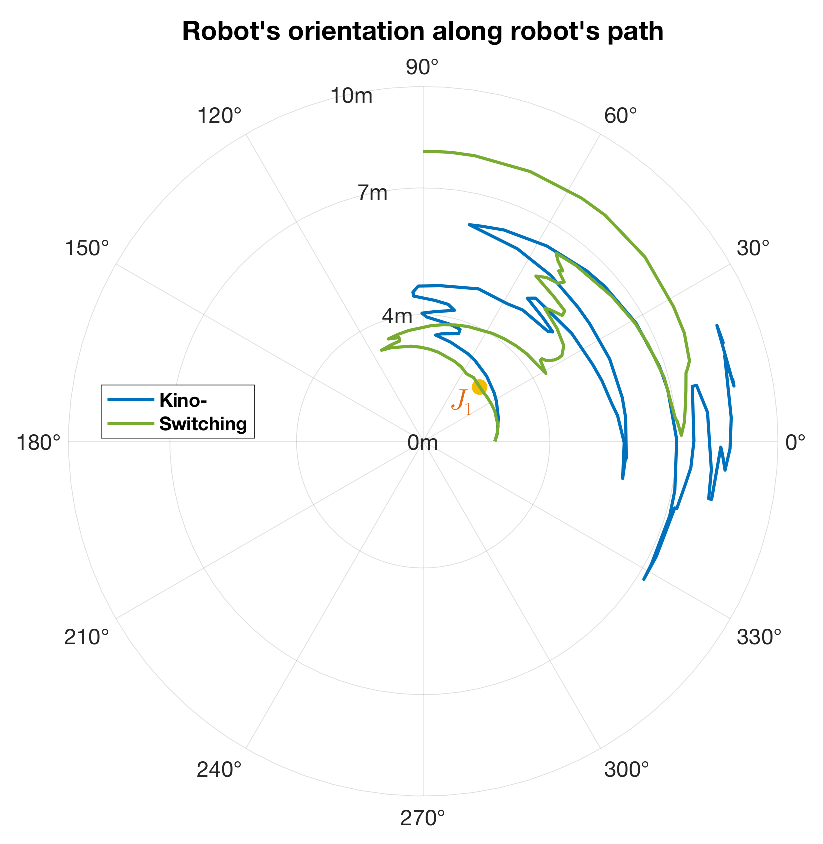
\includegraphics[scale=0.49]{pictures/graphs/sn3_group/sn3_states_pa_1.eps}
				\end{column}
				}
			\only<3>{
				\begin{column}{0.50\textwidth}
					\centering
					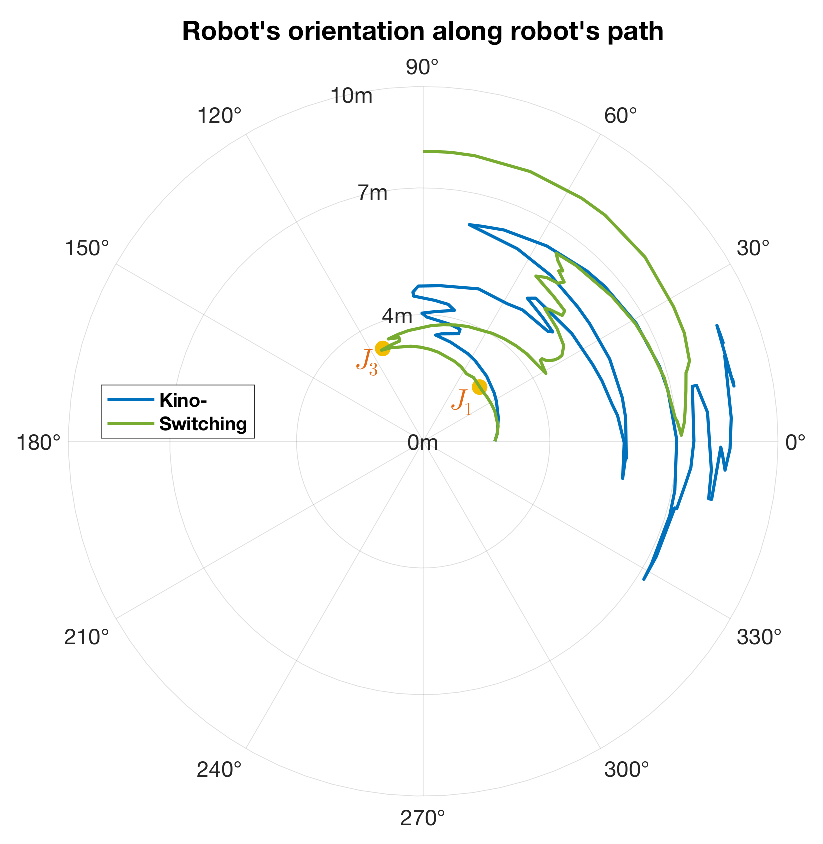
\includegraphics[scale=0.49]{pictures/graphs/sn3_group/sn3_states_pa_2.eps}
				\end{column}
				}
			\only<4>{
				\begin{column}{0.52\textwidth}
					\centering
					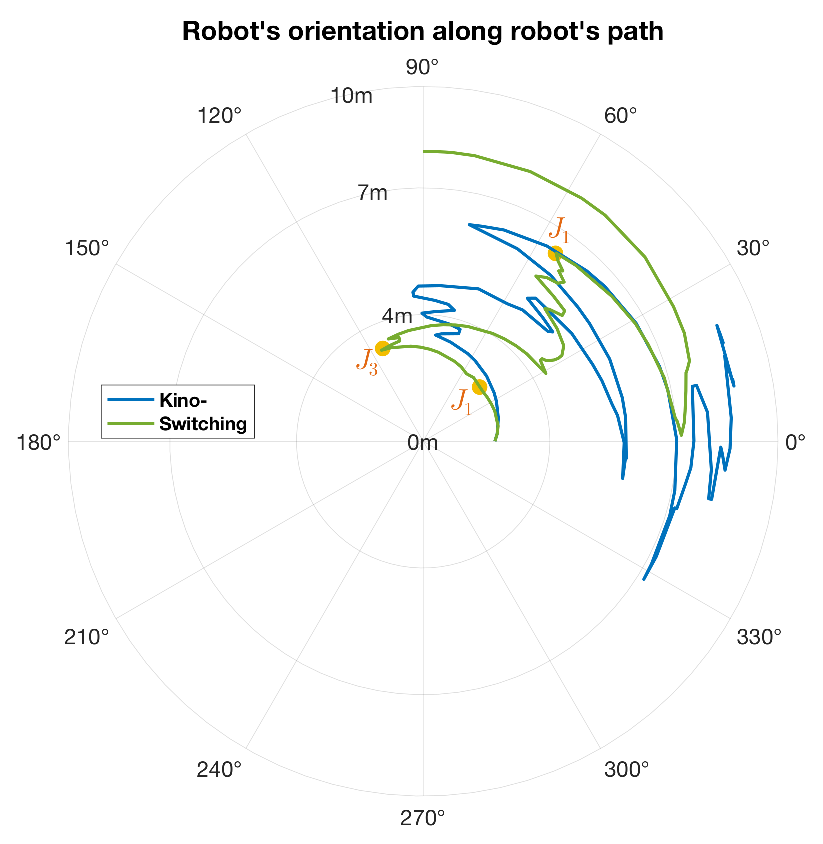
\includegraphics[scale=0.49]{pictures/graphs/sn3_group/sn3_states_pa_3.eps}
				\end{column}
				}
			\only<5>{
				\begin{column}{0.53\textwidth}
					\centering
					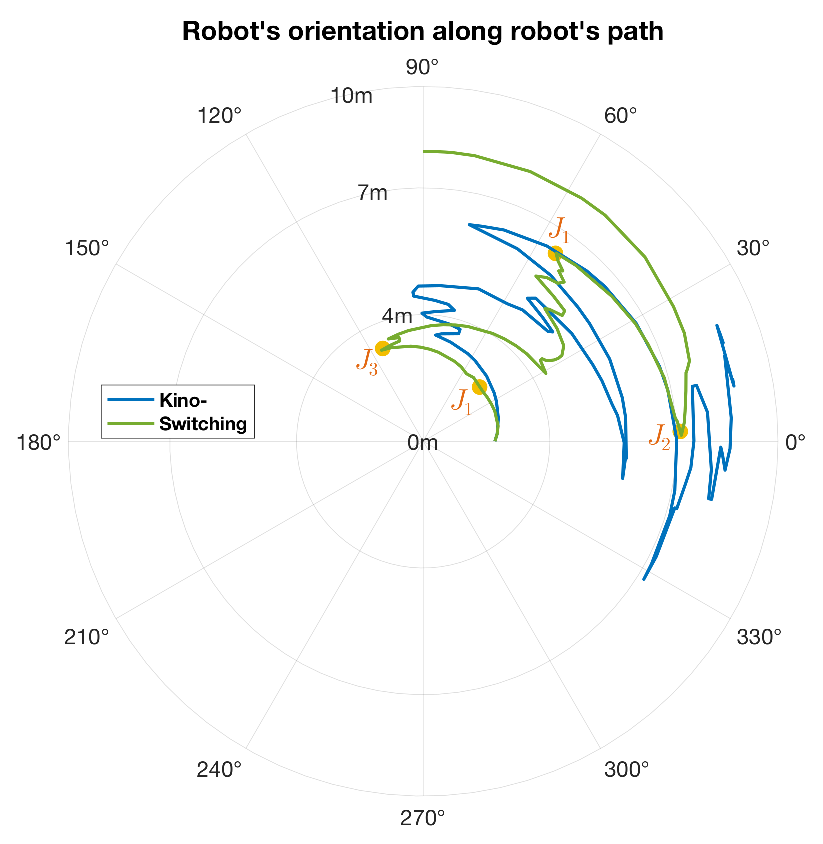
\includegraphics[scale=0.49]{pictures/graphs/sn3_group/sn3_states_pa_4.eps}
				\end{column}
				}
		\end{columns}
	\end{frame}
	
	\begin{frame}
		\frametitle{Scenario \textrm{IV}: Input Trajectory Evolution}
		\only<1>{\centering
			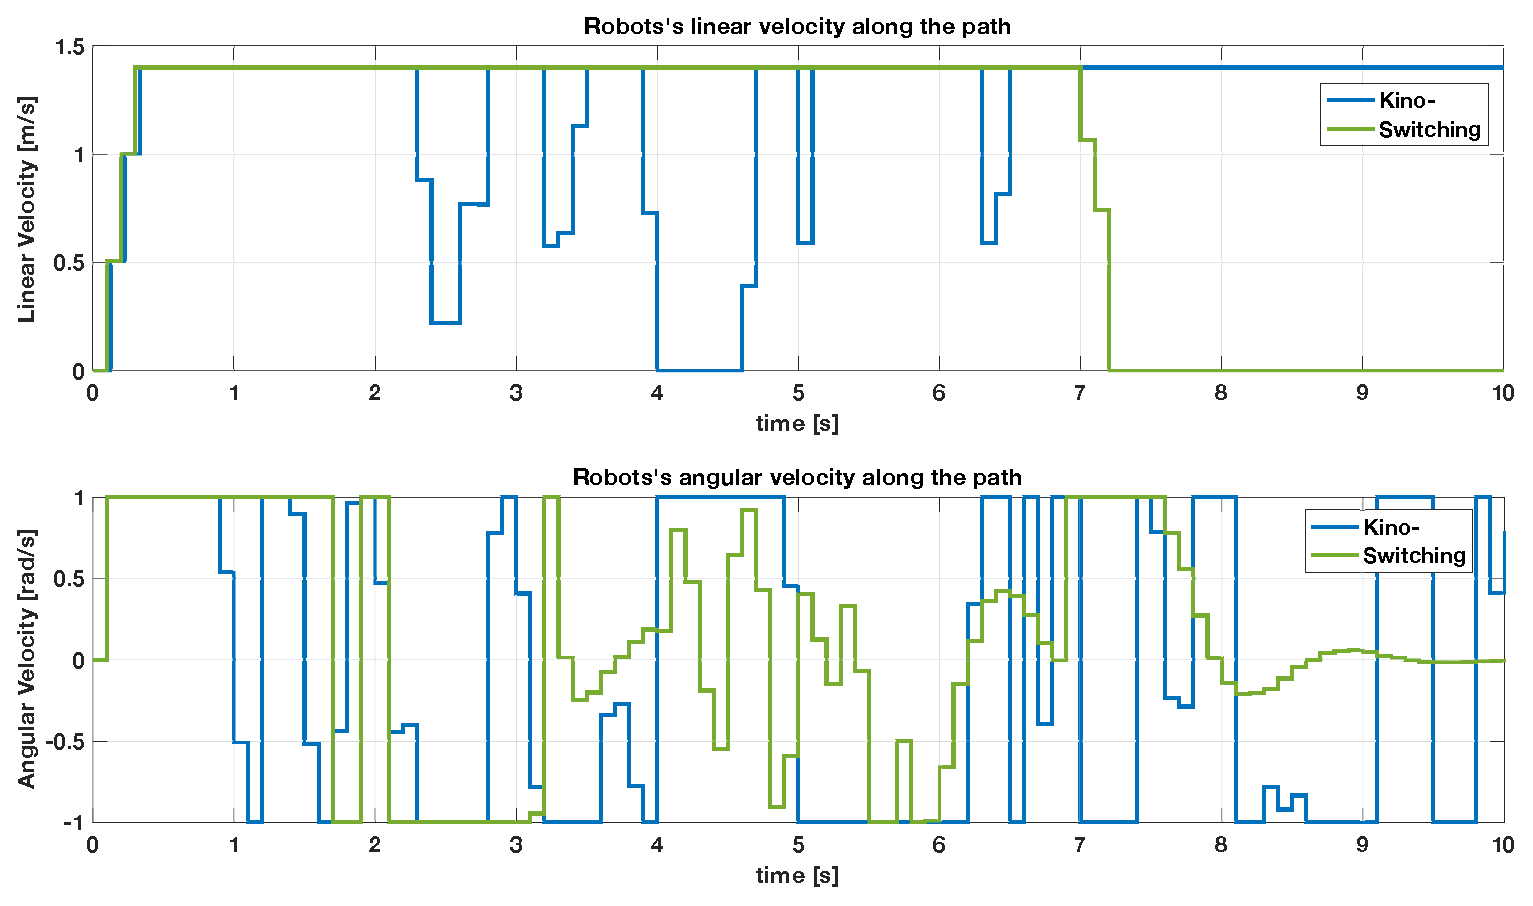
\includegraphics[scale=0.42]{pictures/graphs/sn3_group/sn3_inputs.eps}}
		\only<2>{\centering
			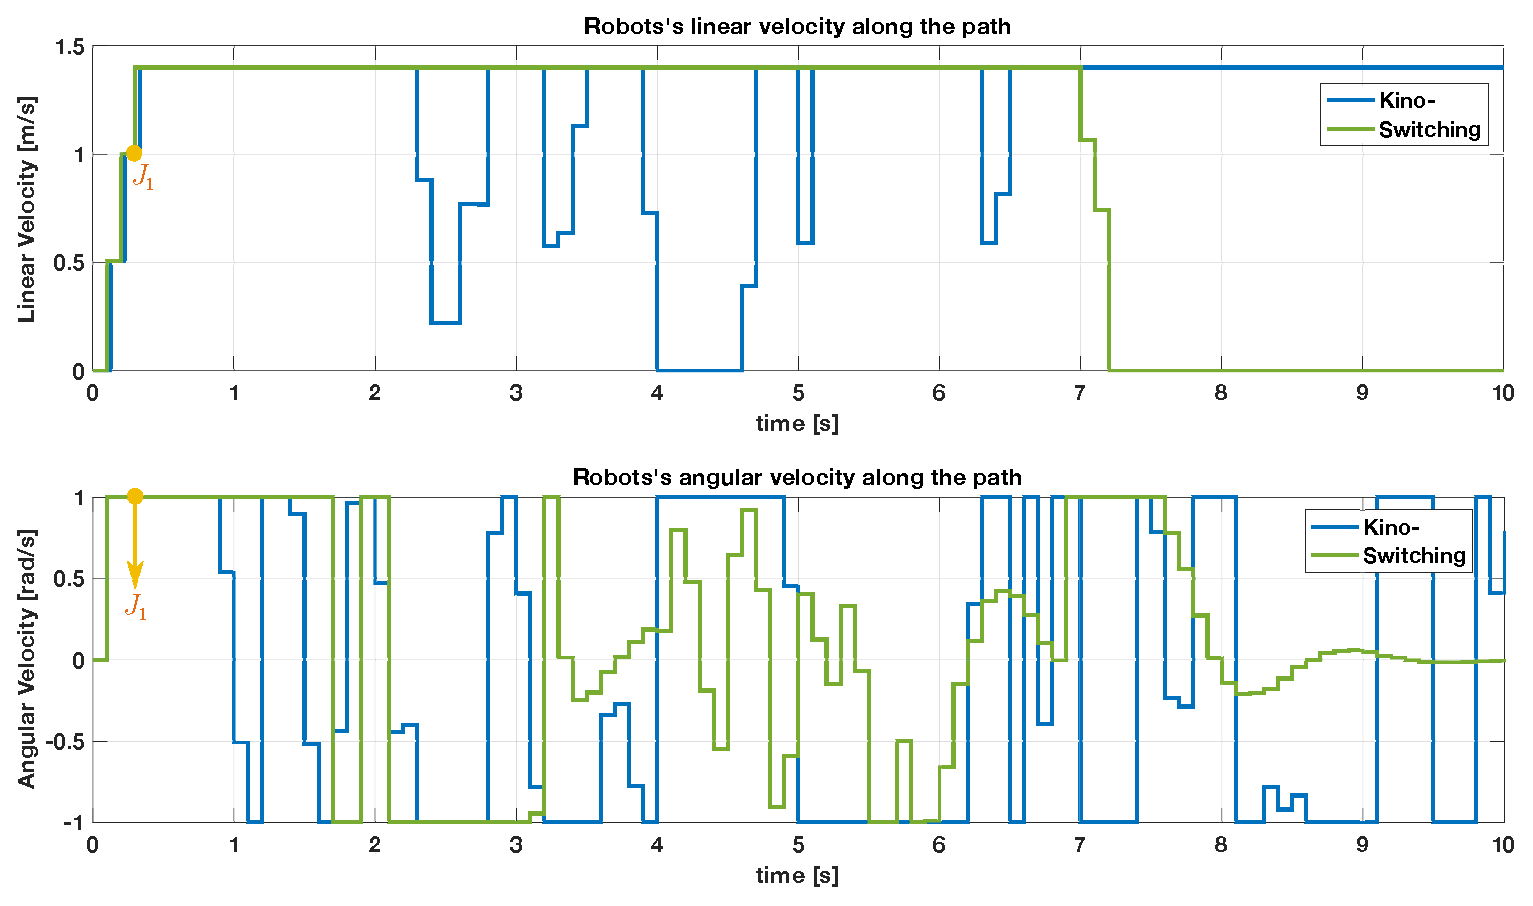
\includegraphics[scale=0.42]{pictures/graphs/sn3_group/sn3_inputs_1.eps}}
		\only<3>{\centering
			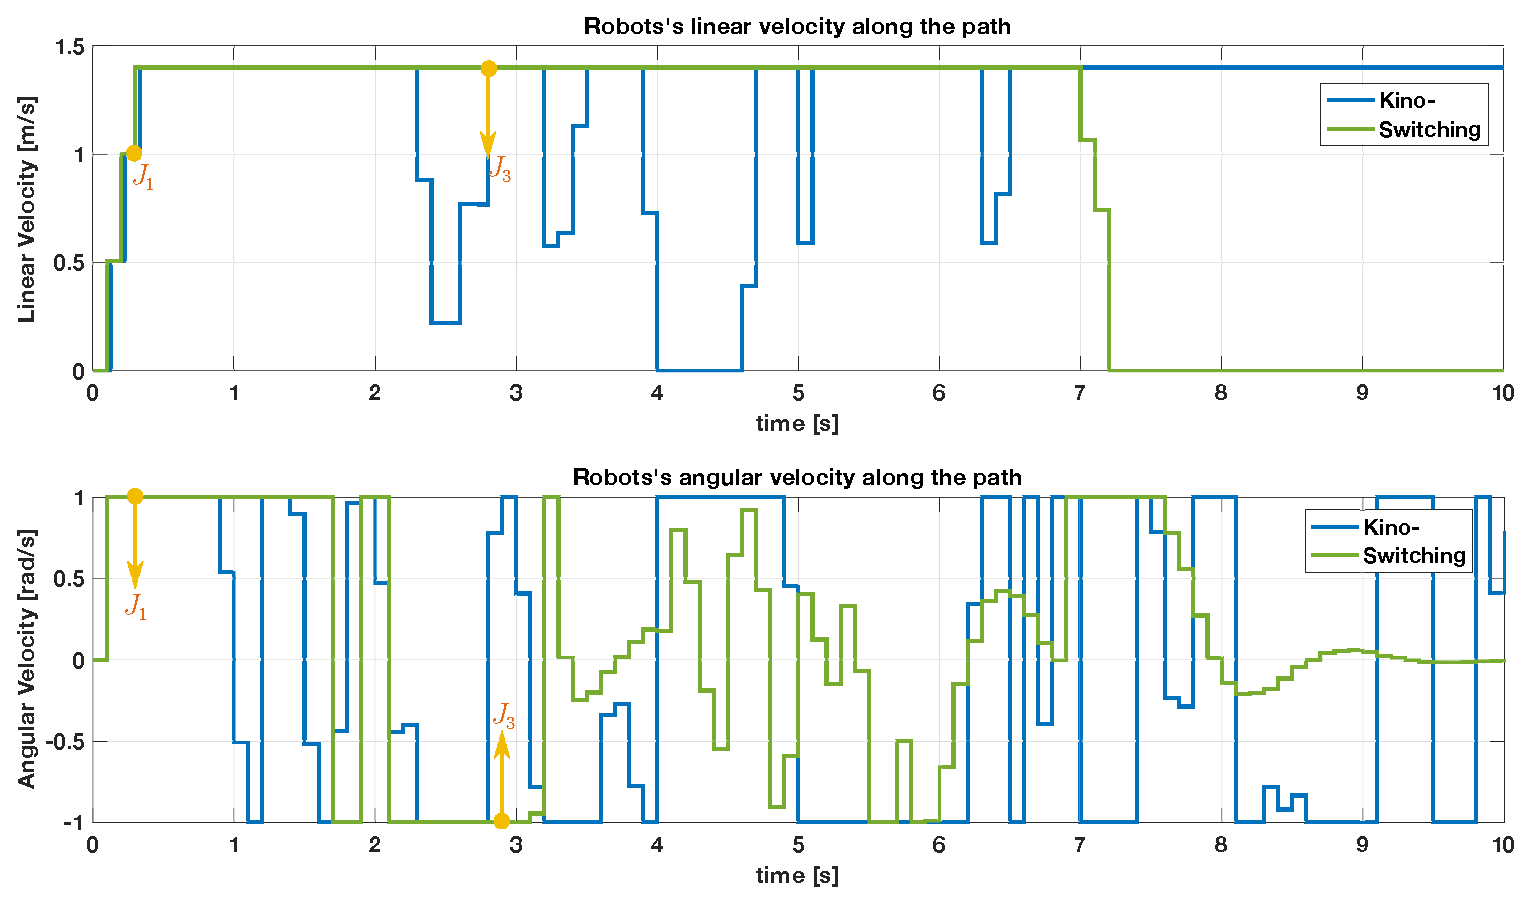
\includegraphics[scale=0.42]{pictures/graphs/sn3_group/sn3_inputs_2.eps}}
		\only<4>{\centering
			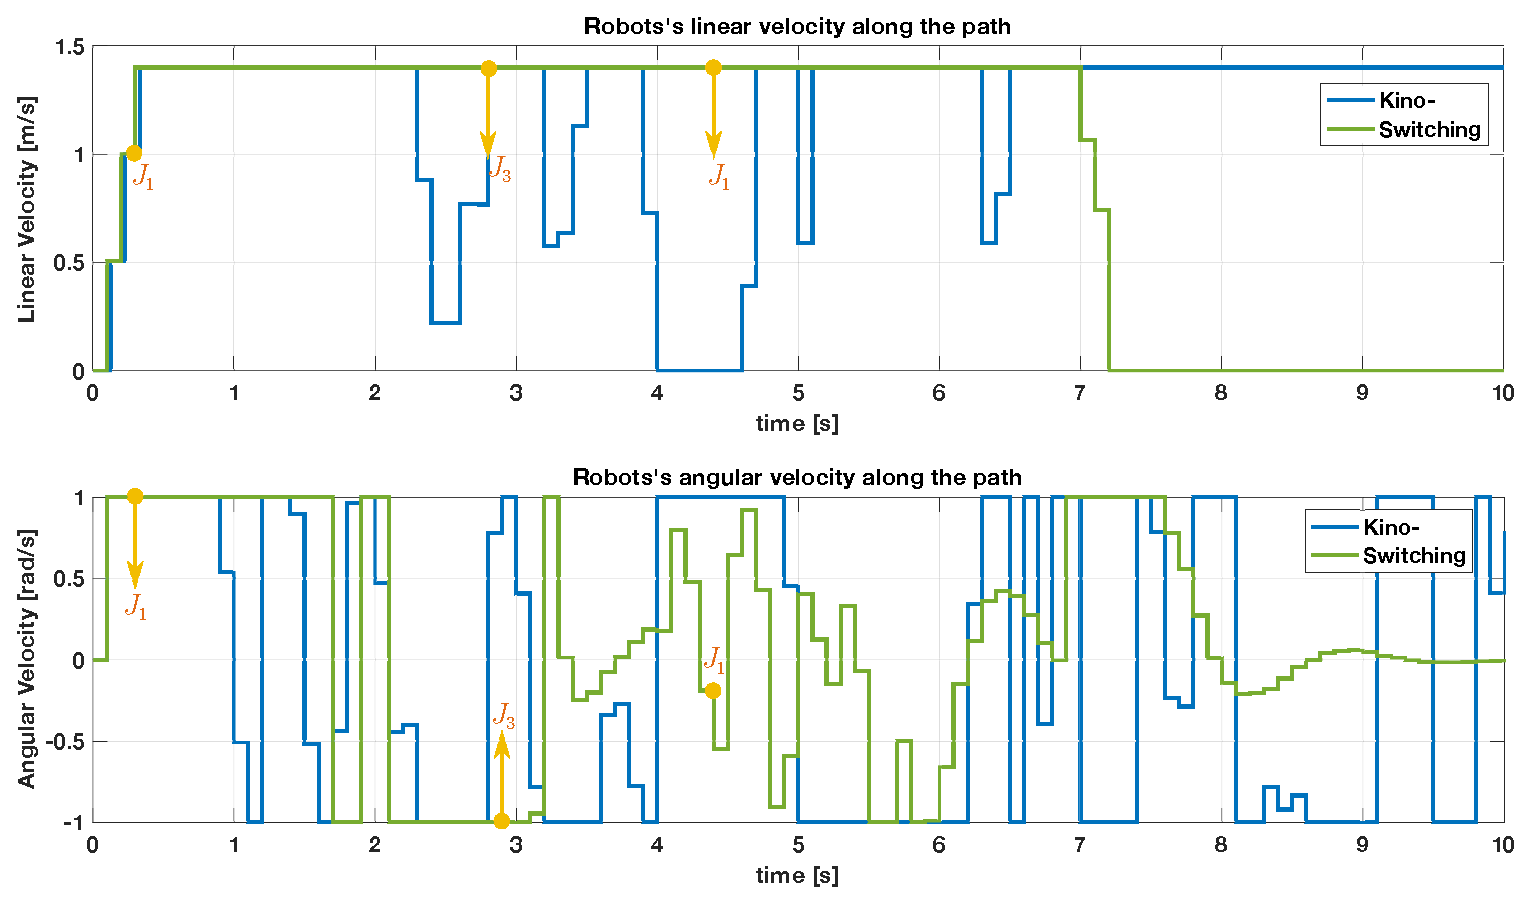
\includegraphics[scale=0.42]{pictures/graphs/sn3_group/sn3_inputs_3.eps}}
		\only<5>{\centering
			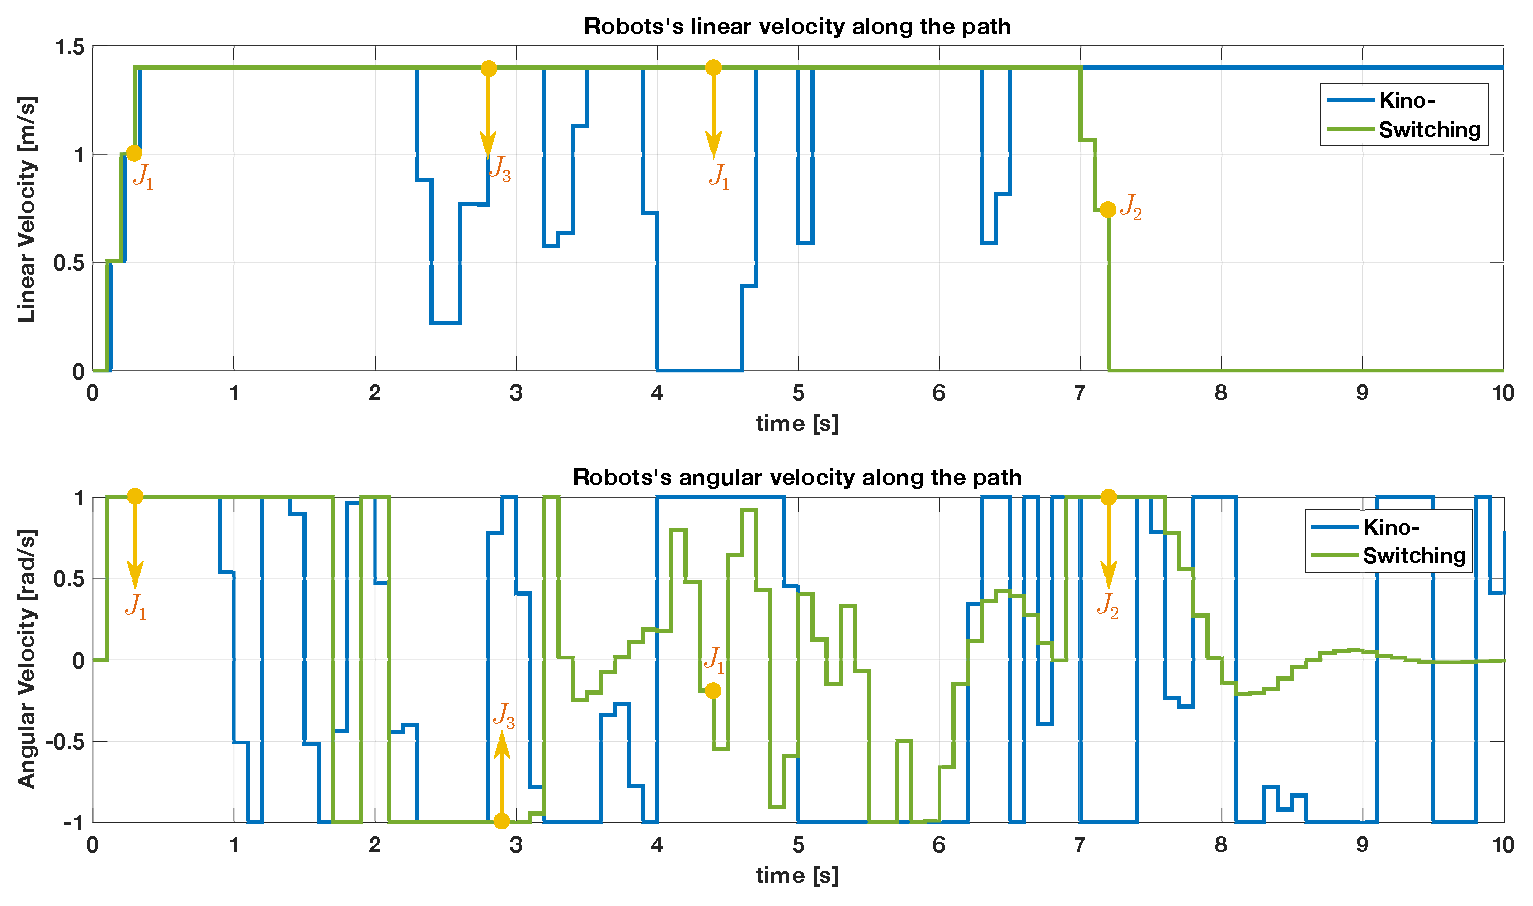
\includegraphics[scale=0.42]{pictures/graphs/sn3_group/sn3_inputs_4.eps}}
	\end{frame}
	
	\begin{frame}
		\frametitle{Scenario \textrm{IV}: NMPC Computational Effort}
		\only<1>{\centering
			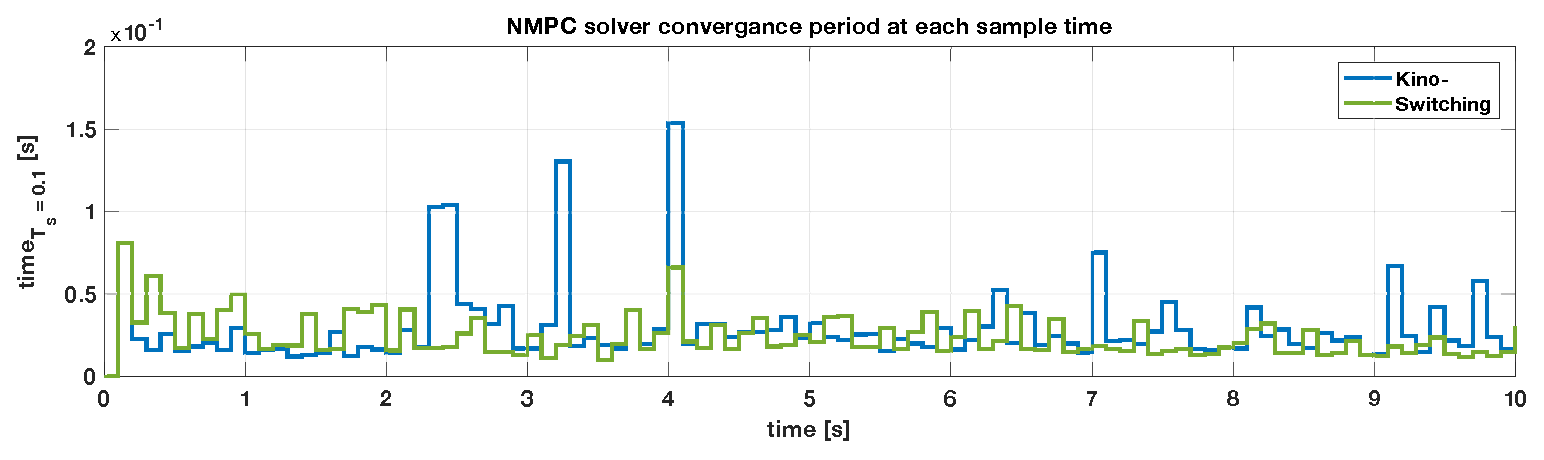
\includegraphics[scale=0.42]{pictures/graphs/sn3_group/sn3_solver_time.eps}}
		\only<2>{\centering
			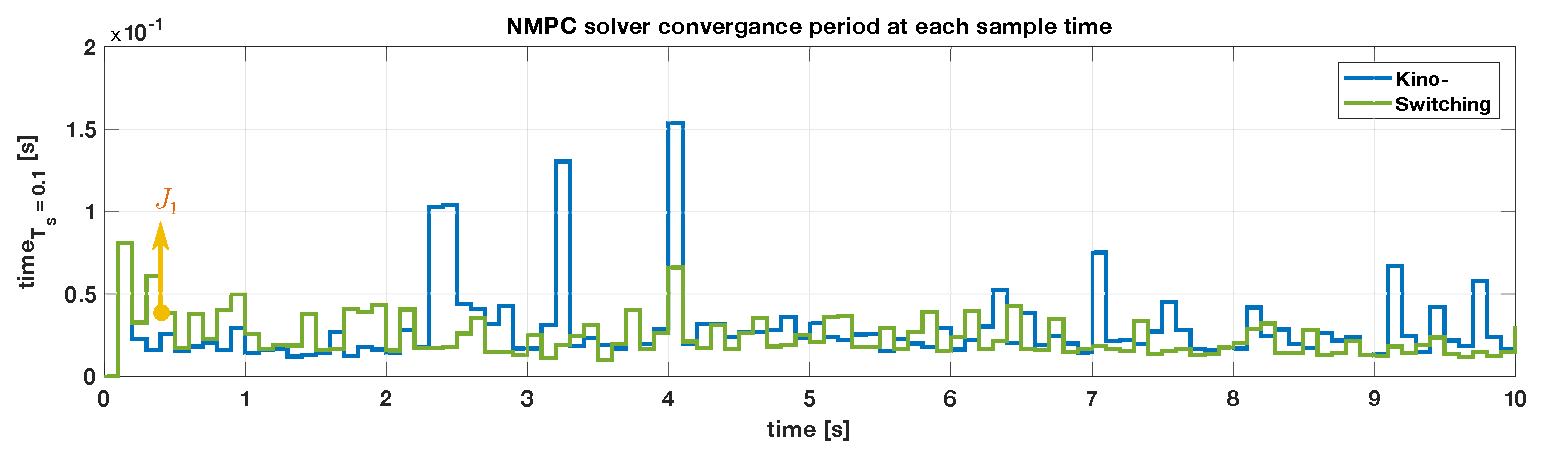
\includegraphics[scale=0.42]{pictures/graphs/sn3_group/sn3_solver_time_1.eps}}
		\only<3>{\centering
			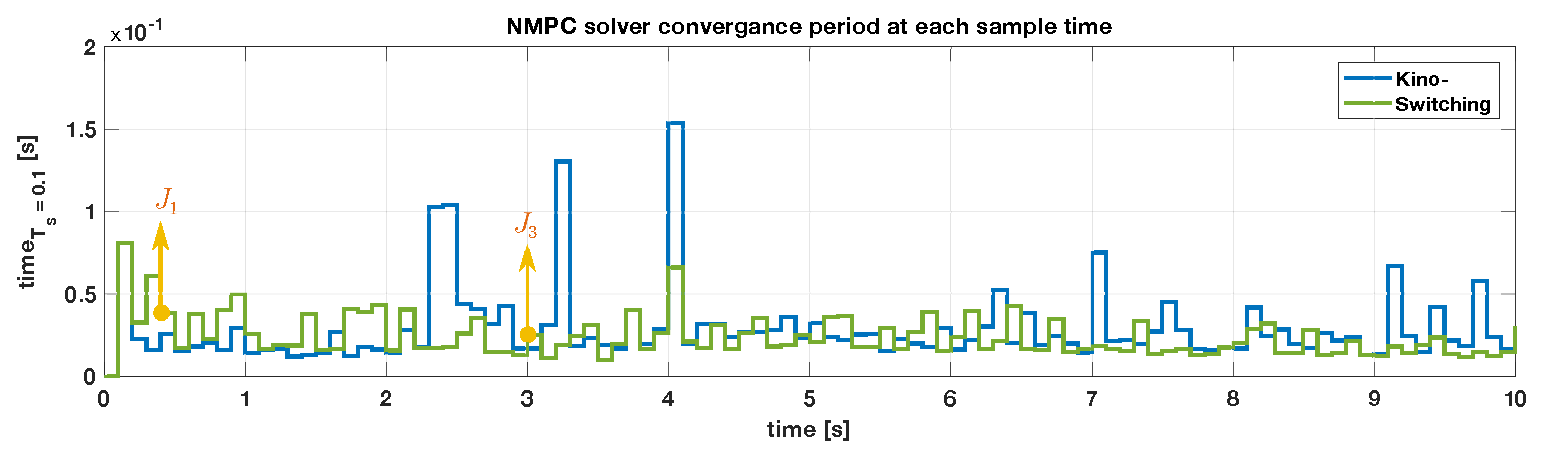
\includegraphics[scale=0.42]{pictures/graphs/sn3_group/sn3_solver_time_2.eps}}
		\only<4>{\centering
			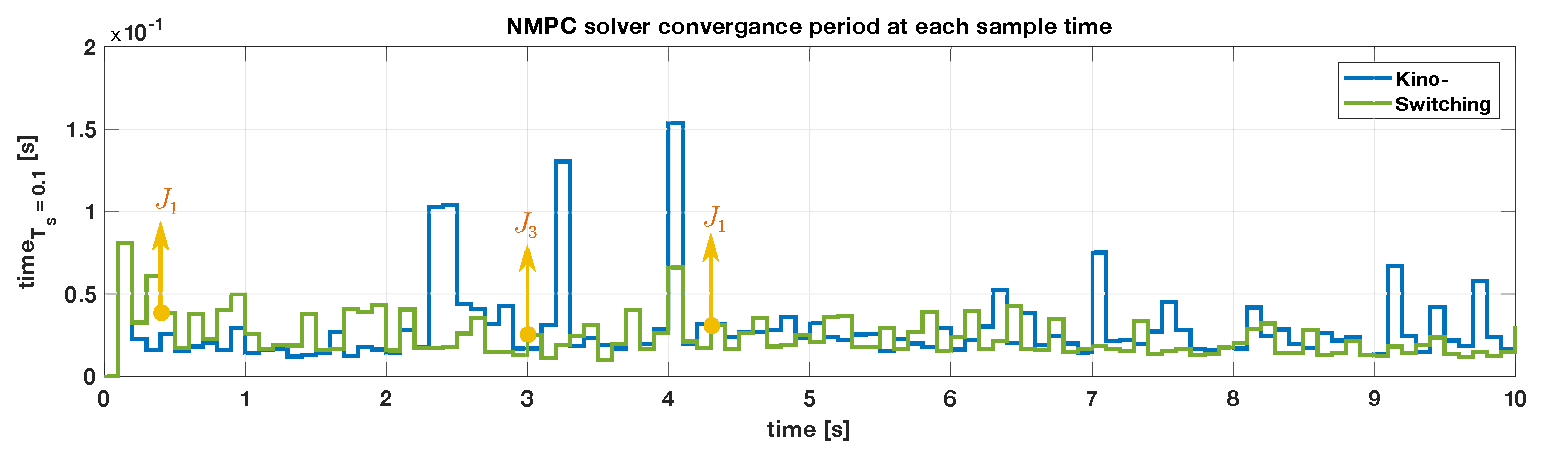
\includegraphics[scale=0.42]{pictures/graphs/sn3_group/sn3_solver_time_3.eps}}
		\only<5>{\centering
			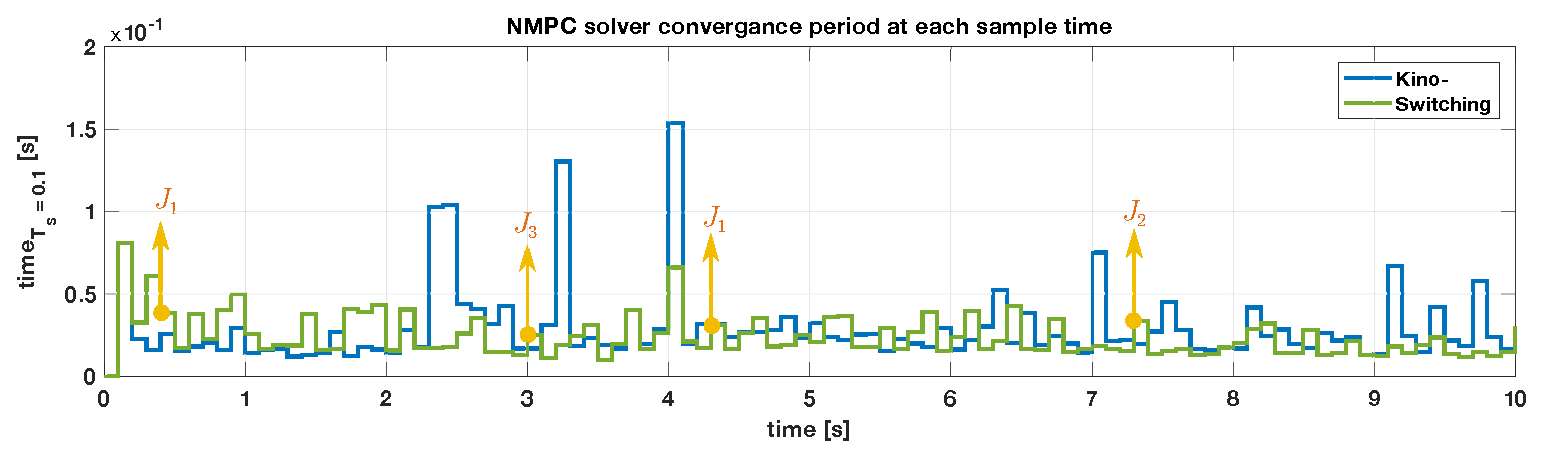
\includegraphics[scale=0.42]{pictures/graphs/sn3_group/sn3_solver_time_4.eps}}
	\end{frame}
	
	\begin{frame}
		\frametitle{Scenario \textrm{IV}: Dynamic Environment}
		\centering
		\movie[width=0.451\textwidth, height=0.9\textheight]
		{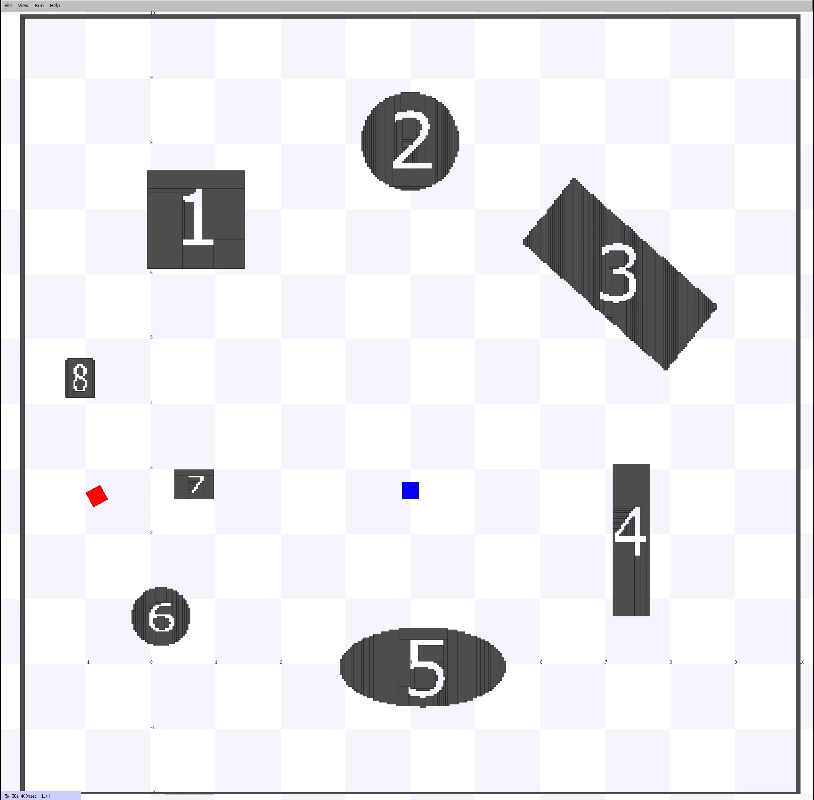
\includegraphics[width=0.45\textwidth]{pictures/good_1.png}}{videos/best.mov}
	\end{frame}

